\section{Auswertung}
\label{sec:Auswertung}

\subsection{Lange Spule}
Im ersten Teil des Versuches wird das Magnetfeld einer langen Spule untersucht. Es wird zuerst die Spule mit der Länge:
\begin{equation*}
l_{\text{S}} = \SI{18,8}{\cm}
\end{equation*}
verwendet und die Messung wird mit:
\begin{equation*}
I = \SI{1}{\ampere}
\end{equation*}
durchgeführt. Die gemessenen Werte für die lange Spule befinden sich in der Tabelle \ref{tab:LangeSpule} und werden in die Abbildung \ref{fig:langespule} eingetragen. Der Anfang der Spule ist bei $x = \SI{0.09}{\meter}$ und die Mitte der Spule ist bei $x = \SI{0.04}{\meter}$. 
\begin{figure}[h!]
	\centering
	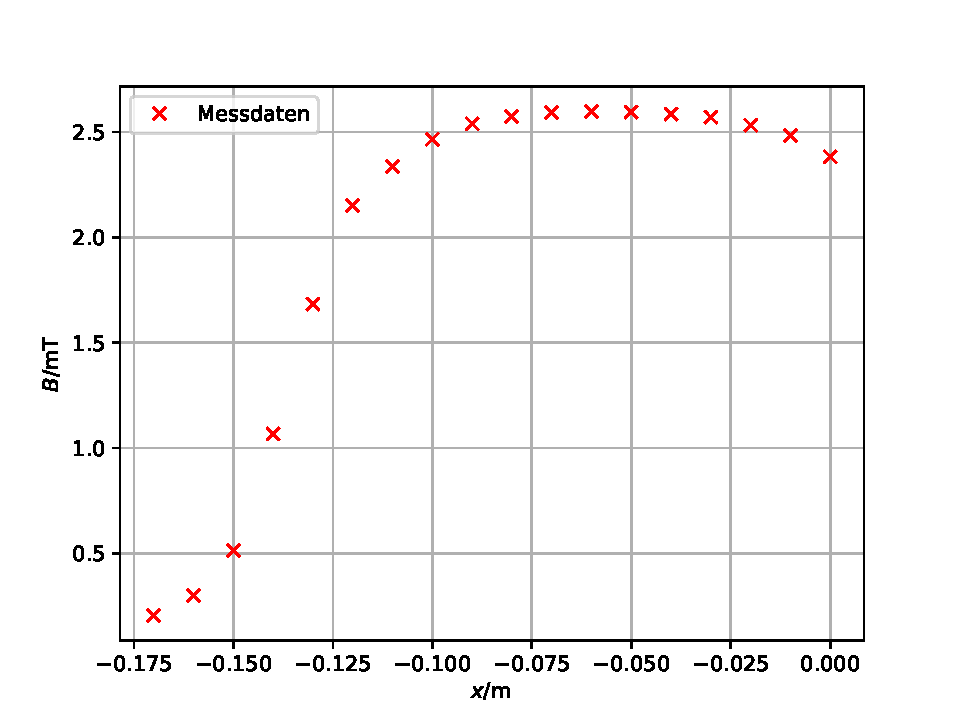
\includegraphics[width=0.7\linewidth]{../../LangeSpule}
	\caption{Das magnetische Feld der langen Spule mit $l_{\text{S}} = \SI{18,8}{\cm}$.}
	\label{fig:langespule}
\end{figure}
\begin{table}[htbp]
	\centering
	\caption{Messdaten zur langen Spule mit $l_{\text{S}} = \SI{18,8}{\cm}$.}
	\label{tab:LangeSpule}
	\begin{tabular}{c c}
		\toprule
		$x / \si{m} $ & $ B / 10^{-3} \si{\tesla}$ \\
		\midrule
		-0,17 & 0,205 \\
		-0,16 & 0,300  \\
		-0,15 & 0,513 \\
		-0,14 & 1,068 \\
		-0,13 & 1,683 \\
		-0,12 & 2,151 \\
		-0,11 & 2,338 \\
		-0,10 & 2,466 \\
		-0,09 & 2,540 \\
		-0,08 & 2,574 \\
		-0,07 & 2,592 \\
		-0,06 & 2,597 \\
		-0,05 & 2,595 \\
		-0,04 & 2,585 \\
		-0,03 & 2,570 \\
		-0,02 & 2,533 \\
		-0,01 & 2,482 \\
	    0 & 2,383 \\
		\bottomrule
	\end{tabular}
\end{table}
\FloatBarrier
Der theoretische Wert berechnet sich mit der Formel \ref{eqn:formel1} und dieser beträgt:
\begin{equation*}
B_{\text{theo}} = \SI{2,005 E-3}{\tesla}.
\end{equation*}
Dabei ist in diesem Fall die magnetische Permeabilität $\mu_{\text{r}} = 1$ und $\mu_{0}$ ist die magnetische Feldkonstante. 
Das Maximum der experimentellen Wert als Vergleich wird mit Hilfe der Messwerten aus der Tabelle \ref{tab:LangeSpule} abgelesen und dieser beträgt:
\begin{equation*}
B_{\text{exp}} = \SI{2,597 E-3}{\tesla}.
\end{equation*}

\subsection{Kurze Spule}
Im zweiten Teil des Versuches wird das Magnetfeld einer kurzen Spulen untersucht. Es wird eine Spule mit der Länge:
\begin{equation*}
l_{\text{k}} = \SI{8,5}{\cm}
\end{equation*}
verwendet und die Messung wird mit:
\begin{equation*}
I = \SI{1}{\ampere}
\end{equation*}
durchgeführt. Die gemessenen Werte für die lange Spule befinden sich im Anhang (siehe \ref{sec:Anhang}) in der Tabelle \ref{tab:KurzeSpule} und werden in die Abbildung \ref{fig:kurzespule} eingetragen. Der Anfang der Spule ist bei $x = \SI{0.15}{\meter} $ und die Mitte der Spule ist bei $x = \SI{0.12}{\meter}$. 
\begin{figure}[h!]
	\centering
	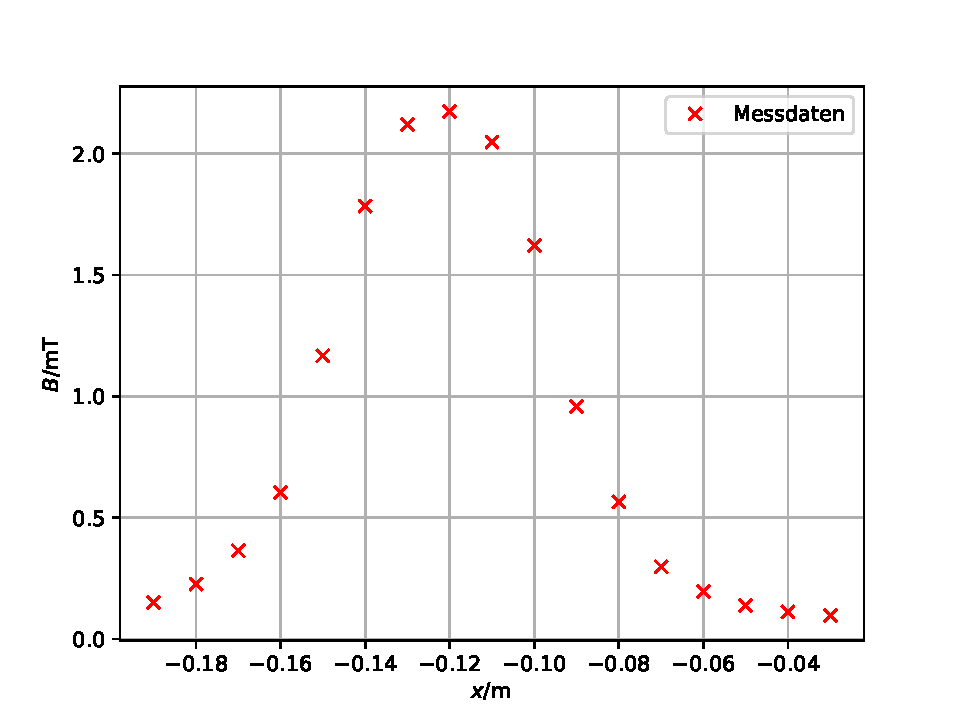
\includegraphics[width=0.7\linewidth]{../../kurzeSpule}
	\caption{Das magnetische Feld der kurzen Spule mit $l_{\text{k}} = \SI{8,5}{\cm}$.}
	\label{fig:kurzespule}
\end{figure}

Der theoretische Wert berechnet sich mit der Formel \ref{eqn:formel1}  und dieser beträgt:
\begin{equation*}
B_{\text{theo}} = \SI{4,435 E-3}{\tesla}.
\end{equation*}
Dabei ist in diesem Fall die magnetische Permeabilität $\mu_{\text{r}} = 1$ und $\mu_{0}$ ist die magnetische Feldkonstante. 
Das Maximum der experimentellen Wert als Vergleich wird mit Hilfe der Messwerten aus der Tabelle \ref{tab:KurzeSpule} abgelesen und dieser beträgt:
\begin{equation*}
B_{\text{exp}} = \SI{2,174 E-3}{\tesla}.
\end{equation*}

\subsection{Magnetfeld eines Helmholtzspulenpaares}
An dieser Stelle werden die magnetischen Flussdichte auf der Symmetrieachse des Helmholtzspulenpaares für drei verschiedene Abstände näher untersucht. Mit der Messaparatur muss einen minimalen Abstand von $\SI{7}{\cm}$ eingestellt werden, deshalb liegen die Spulenabstände bei $d_{1} = \SI{7}{\cm}$ , $d_{2} = \SI{9}{\cm}$ und $d_{3} = \SI{11}{\cm}$. Die Spulen haben einen Radius von $r = \SI{0,125}{\meter}$. 

\subsubsection{Erster Abstand}
Die Messwerte innerhalb und außerhalb der Helmholtzspulenpaare zur ersten Abstand befinden sich im Anhang (siehe \ref{sec:Anhang})  in der Tabelle \ref{tab:ErsterAbstand} und diese werden in die Abbildung \ref{fig:abstand1} eingetragen. 
\begin{figure}[h!]
	\centering
	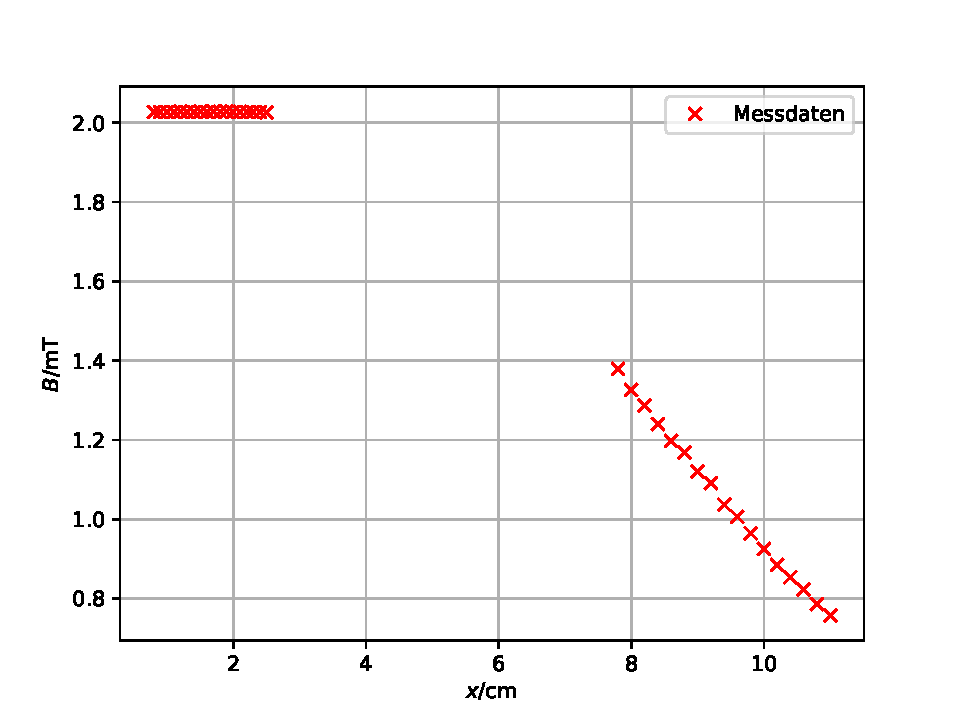
\includegraphics[width=0.7\linewidth]{../../Abstand1}
	\caption{Graphik des Magnetfeldes für eine Helmholtzspule bei einem Abstand von $d_{1} = \SI{7}{\cm}$.}
	\label{fig:abstand1}
\end{figure}

Der theoretische Wert berechnet sich mit der Formel \ref{eqn:formel2} und beträgt:
\begin{equation*}
B_{\text{theo1}} = \SI{1,201 E-3}{\tesla}.
\end{equation*}
Für den experimentellen Wert ergibt sich:
\begin{equation*}
B_{\text{exp1}} = \SI{1,575 E-3}{\tesla}.
\end{equation*}

\subsubsection{Zweiter Abstand}
Die Messwerte innerhalb und außerhalb der Helmholtzspulenpaare zur zweiten Abstand befinden sich im Anhang (siehe \ref{sec:Anhang}) und diese werden in die Abbildung \ref{fig:abstand2} eingetragen. 
\begin{figure}[h!]
	\centering
	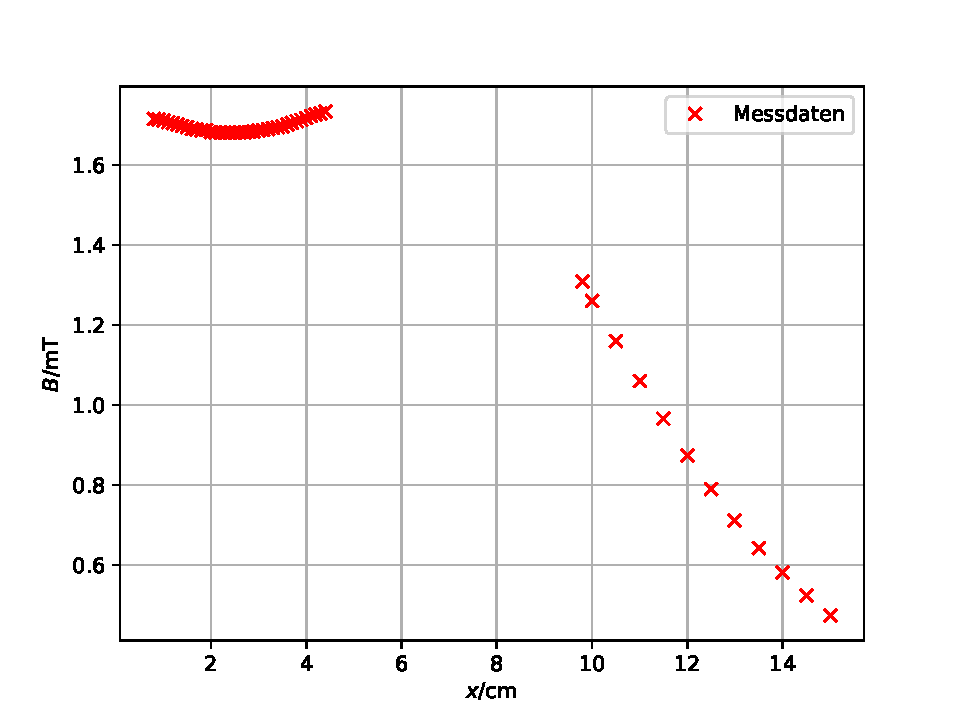
\includegraphics[width=0.7\linewidth]{../../Abstand2}
	\caption{Graphik des Magnetfeldes für eine Helmholtzspule bei einem Abstand von $d_{2} = \SI{9}{\cm}$.}
	\label{fig:abstand2}
\end{figure}

Der theoretische Wert berechnet sich mit der Formel \ref{eqn:formel2} und beträgt:
\begin{equation*}
B_{\text{theo2}} = \SI{1,074 E-3}{\tesla}.
\end{equation*}
Für den experimentellen Wert ergibt sich:
\begin{equation*}
B_{\text{exp2}} = \SI{1,268 E-3}{\tesla}.
\end{equation*}

\subsubsection{Dritter Abstand}
Die Messwerte innerhalb und außerhalb der Helmholtzspulenpaare zur dritten Abstand befinden sich im Anhang (siehe \ref{sec:Anhang}) und diese werden in die Abbildung \ref{fig:abstand3} eingetragen. 
\begin{figure}[h!]
	\centering
	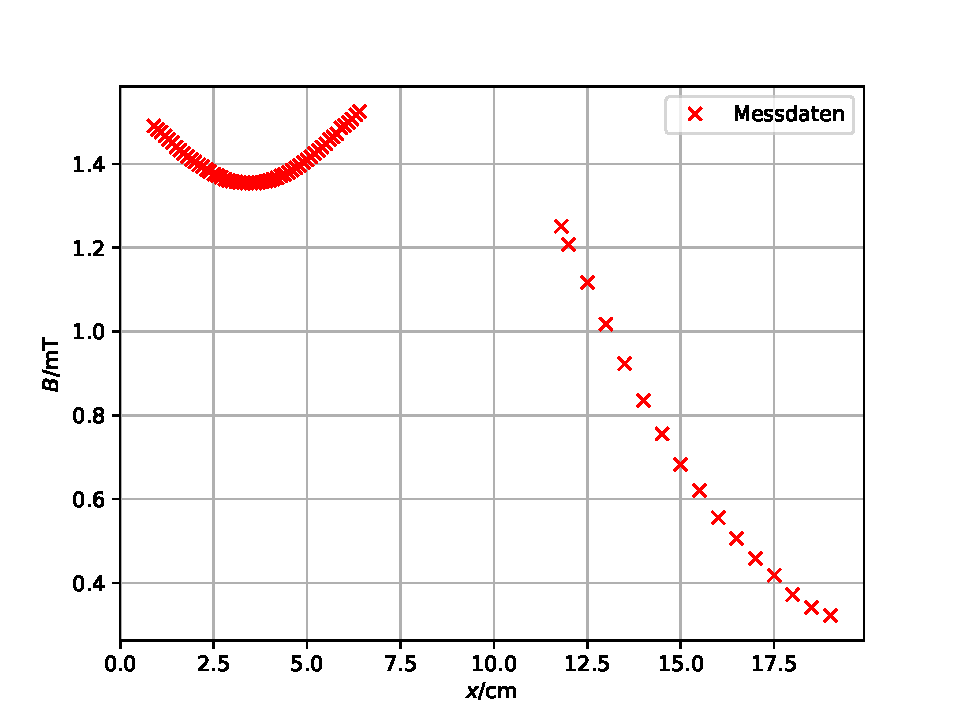
\includegraphics[width=0.7\linewidth]{../../Abstand3}
	\caption{Graphik des Magnetfeldes für eine Helmholtzspule bei einem Abstand von $d_{3} = \SI{11}{\cm}$.}
	\label{fig:abstand3}
\end{figure}

Der theoretische Wert berechnet sich mit der Formel \ref{eqn:formel2} und beträgt:
\begin{equation*}
B_{\text{theo3}} = \SI{8,506 E-4}{\tesla}.
\end{equation*}
Für den experimentellen Wert ergibt sich:
\begin{equation*}
B_{\text{exp3}} = \SI{3,320 E-4}{\tesla}.
\end{equation*}

\subsection{Hysteresekurve}
Im letzten Versuchsteil wird eine Toroidspule mit Eisenkern betrachtet. Die magnetische Flussdichte wird für einen ansteigenden und abfallenden Strom aufgenommen und in der Tabelle aus der Kapitel \ref{sec:Anhang} notiert. Die Messwerten werden anschließen in die Abbildung \ref{fig:hysterese} eingetragen.

\begin{figure}[h!]
	\centering
	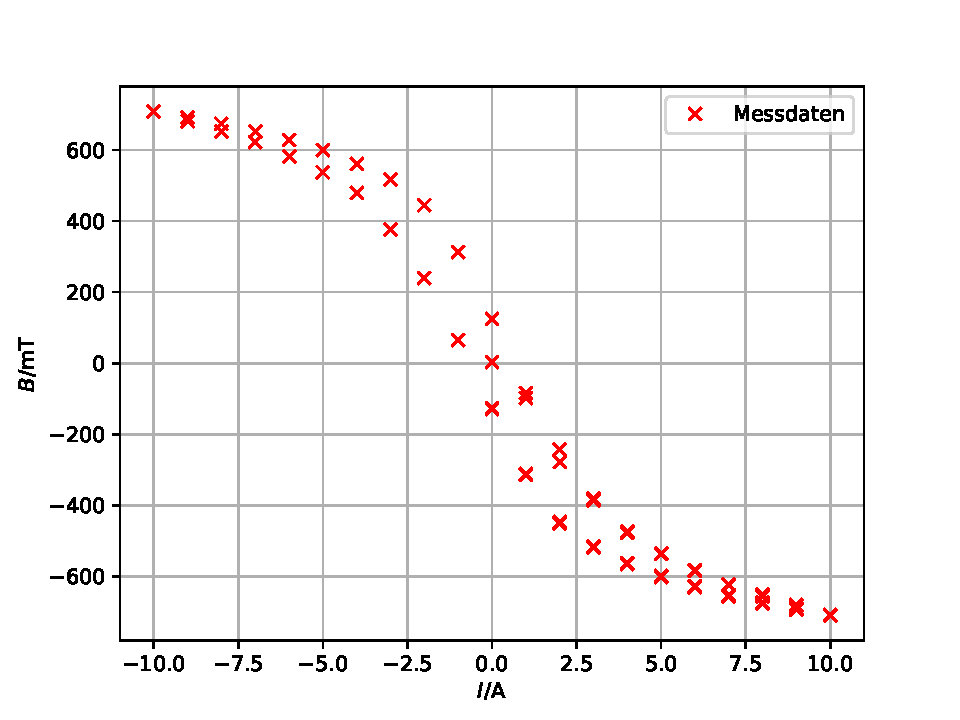
\includegraphics[width=0.7\linewidth]{../../Hysterese}
	\caption{Hysteresekurve zur letzten Messung.}
	\label{fig:hysterese}
\end{figure}

Aus der Abbildung \ref{fig:hysterese} lassen sich die Werte für die Remanenz $B_{\text{r}}$, den Sättigungswert $B_{\text{s}}$ sowie die Koerzitivkraft $H_{\text{c}}$ ablesen. Für die Remanenz muss $B_{\text{r}} (H=0) \neq 0$ gelten und somit folgt:
\begin{equation*}
B_{\text{r}} = \SI{-127,1}{\milli\tesla}.
\end{equation*}

Die Hysteresekurve strebt mit abnehmender magnetischen Feldstärke einen Sättigungswert an und aus der Abbildung \ref{fig:hysterese} folgt:
\begin{equation*}
B_{\text{s}} = \SI{-710,2}{\milli\tesla}.
\end{equation*}

Für die Koerzitivkraft wird folgendes abgelesen:
\begin{equation*}
H_{\text{c}} = \SI{-0,5}{\ampere}.
\end{equation*}